\chapter*{Introduction}
\addcontentsline{toc}{chapter}{Introduction}

Source code documentation is an essential part of any quality project \cite{rachel_why_2018}. Unfortunately, writing and keeping such documentation up to date is often overlooked or inconvenient for various reasons, such as strict deadlines. That might lead to the degradation of project quality, as developers who leave said projects usually take their know-how with them without properly passing it down to their replacements.

In cases where source code documentation has a higher priority than usual, extracting said documentation from the source code into a searchable, public format such as \ref{itm:html} is good practice \cite{smrita_benefits_2014}. Documentation-generating tools accomplish that. The primary benefit of this practice is the resulting comprehensive overview of the source code, accessible to interested parties \cite{smrita_benefits_2014}.

For Microsoft \ref{gloss:dotnetlabel} projects, there is a selection of documentation-generating tools available, which includes: DocFX, Doxygen, SourceBrowser, and others \cite{wagner_xml_2022}. These solutions primarily generate output in \ref{itm:html}, which is sufficient for most projects. However, these tools often lack support for output formats like \ref{itm:pdf}, \ref{gloss:markdown}, or custom. Moreover, the customization of these tools is minimal, preventing projects from being able to fit such tools to their exact needs. Furthermore, their \ref{itm:ui}/\ref{itm:ux} leaves much to be desired, introducing an unnecessary learning curve and lowering usability.

With that in mind, there is visible room for improvement. A desirable documentation-generating tool would be easy to use, modern, extensible, rich in output format support, and performant. Satisfying the desires of an modern extensible application requires the thorough use of programming design patterns \cite{humblot_design_2021} such as \ref{itm:solid} \cite{hall_adaptive_2017}, \ref{itm:di} \cite{deursen_dependency_2019}, and \ref{itm:mvvm} \cite{katz_mvvm_2022}.

\section*{Motivation}
\addcontentsline{toc}{section}{Motivation}

The motivation for creating a custom tool is primarily a personal need to provide easy access to code documentation. Since most open-source projects are hosted either on GitHub.com or GitLab.com \cite{alphabet_inc_google_2022}, it makes sense to utilize said platforms built-in wiki pages for hosting source code documentation for consistency. However, a minority of developers use Bitbucket to host their public open-source projects \cite{jiricek_why_2022}, as this platform targets the enterprise market. Additionally, corporate clients who purchase Bitbucket usually consider using Confluence alongside it, which serves as a documentation hosting platform. That is because both products are from the same vendor, Atlassian. Directly supporting Bitbuckets wiki is not a priority; however, adding future support for Confluence is possible, given the tool's extensibility.

When attempting to find existing solutions for generating documentation, none had the desired extensibility and were mainly limited to creating static \ref{itm:html} pages.
Since the central \ref{gloss:git} hosting platform's wiki pages predominantly utilize \ref{gloss:markdown} for displaying formatted text\footnote{Apart from \ref{gloss:markdown}, said \ref{gloss:git} platforms support more formats; however, the latter has the richest formatting capabilities}, static \ref{itm:html} pages are out of the question.

Thus, the idea of developing a custom tool that would create \ref{gloss:markdown} documentation from \ref{gloss:dotnetlabel} libraries for \ref{gloss:git} platforms came to fruition. Nevertheless, focusing only on one output format would waste of time and effort, as only some would need such a tool. Thus, the result of the development should be a generic tool that allows anyone to modify it to output to any desirable format.

Conducting a questionnaire to identify developer needs for documentation-generating tools in the \ref{gloss:dotnetlabel} world supported this motivation. The questionnaire result (see section \ref{sec:whatdouserswant}) confirmed a generally low interest in writing documentation; however, it highlighted the desires of those few developers who do care about maintaining source code documentation.

\section*{Goal}
\addcontentsline{toc}{section}{Goal}

This thesis aims to create a custom documentation-generating tool for \ref{gloss:dotnetlabel} projects using appropriate design patterns such as \ref{itm:solid}, \ref{itm:di}, and \ref{itm:mvvm}, and to satisfy user needs for extensibility, ease of use, modern design, and support for many output formats. Furthermore, reaching the goal must not introduce worse performance than existing tools.

Based on an analysis of currently available documentation tools (see section \ref{sec:whatisavailable}), developer needs (see section \ref{sec:whatdouserswant}), personal experience, and general project development guidelines, the following milestones are defined:
\begin{enumerate}
    \item Proof of concept
    \item Evaluation and project planning
    \item Processing libraries
    \item \ref{itm:gui} application
    \item \ref{gloss:markdown} for \ref{gloss:git} plugin
\end{enumerate}

Achieving each one is a step closer to the end goal of a functioning custom documentation-generating tool.

\subsection*{Proof of concept} \label{subSecProofOfConcept}
\addcontentsline{toc}{subsection}{Proof of concept}

Creating a proof of concept program will help understand whether the project is realistic, what challenges will occur and how to overcome them.
The main drawback of this is that it will take additional time; however, the gained perspectives are quintessential for the correct project planning.

The focus of this milestone is to find out how to extract the necessary data for documentation generation and attempt to generate said documentation.
That is needed because no existing reference project could provide the required guidelines in a reasonable amount of time.
All other requirements based on the takeaways from the survey (see \ref{ssec:questionnaireeval}) can be omitted from this stage, as reference projects and personal experience is available.

\subsection*{Evaluations and project planning} \label{subSecEvalProjPlanning}
\addcontentsline{toc}{subsection}{Evaluations and project planning}

Concise planning of the project, based on the gained experience from the proof of concept, will, as a result, yield a higher quality product.
Extensibility will be the key feature of the project. Therefore, careful planning of the code structure is required to avoid unnecessary complications.
Meanwhile, the planning phase should not take unreasonable effort, as the ratio of time spent to results will diminish over time (as seen in figure \ref{fig:overplanning}) \cite{ruparelia_stop_2016}.

\begin{figure}[H]
    \centering
    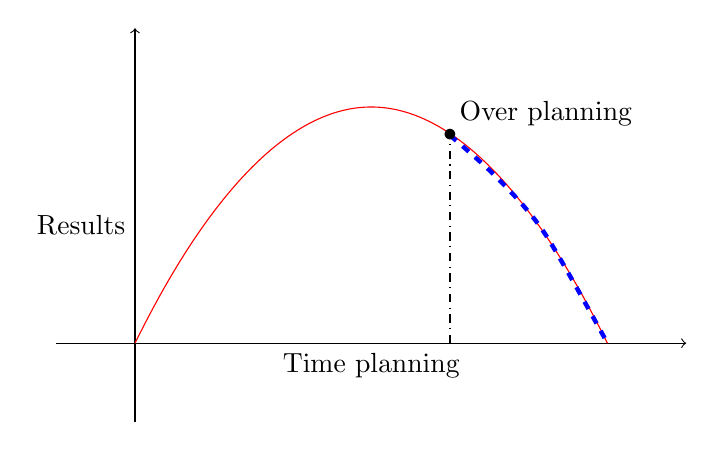
\begin{tikzpicture}
        \draw [->] (-4, 0)--(4,0) node [midway, below]{Time planning};
        \draw [->] (-3, -1)--(-3,4) node[left, midway]{Results};

        \draw [red] (0, 3) parabola(-3,0); % Left
        \draw [red] (0, 3) parabola(3,0); % Right
        \draw [ultra thick, blue, dashed] plot [smooth] coordinates {(1, 2.64) (1.6,2.1) (2.2, 1.40) (3, 0)}; % Right

        \draw [dash dot] (1,0)--(1, 2.64);

        \draw (1, 2.64) node [above right]{Over planning};
        \draw (1, 2.64) node {$\bullet$};
    \end{tikzpicture}
    \caption{Overplanning visualized}
    \label{fig:overplanning}
\end{figure}

This milestone aims to gain a clear picture of what techniques, design patterns \cite{humblot_design_2021}, and technologies should be used or avoided to satisfy all project requirements with minimum compromise.

\subsection*{Processing libraries} \label{subSecProcessingLibs}
\addcontentsline{toc}{subsection}{Processing libraries}

The focus of this milestone will be creating processing libraries that will serve as the application's core. Said libraries will take some input and provide the output necessary for generating the desired documentation. The types of libraries and their implementation depend on the previous milestones. The result of this milestone will be a set of working libraries.

\subsection*{GUI application} \label{subSecGuiApp}
\addcontentsline{toc}{subsection}{GUI application}

The \ref{itm:gui} application will serve as the façade for users utilizing the tool. Said application must be cross-platform, have a modern design, and provide as seamless a user experience as possible, considering the extensible nature of the tool.

Thus, this milestone aims to create such a \ref{itm:gui} façade that will have a simple, yet functional \ref{itm:ux}/\ref{itm:ui}. Additional goals might be added based on the outcomes of previous milestones.

\subsection*{Markdown for Git plugin} \label{subSecMdGitPlugin}
\addcontentsline{toc}{subsection}{Markdown for Git plugin}

Creating the first plugin for the tool will be the final milestone for the time being as its creation reaches the goal of this thesis.
The plugin will be composed of the processing libraries created in the fourth milestone.

The goal is to create a plugin that can be distributed separately from the main application. That would allow users to choose what plugins they wish to use and omit to install ones they do not.
